\chapter{Alternating Currents}

\section{Alternating Currents}

\begin{definition}
    An \vocab{alternating current} is an electric current that periodically reverses its direction in a circuit.
\end{definition}

\begin{definition}
    The \vocab{peak value} ($I_0$) is the maximum absolute value of the alternating current or voltage in either direction of zero value in a periodic cycle.
\end{definition}

\begin{definition}
    The \vocab{peak-to-peak value} is the difference between the positive peak value and the negative peak value of the alternating current within a cycle.
\end{definition}

\begin{definition}
    The \vocab{root-mean-square} ($I_{\text{rms}}$) value of an alternating current is the value of the steady direct current that dissipates energy at the same average rate as the alternating current.
\end{definition}

Mathematically, \[I_{\text{rms}} = \sqrt{\frac1T \int_0^T I^2 \d t}.\]

\begin{proposition}
    The mean power $\ba{P}$ dissipated in a load $R$ by an alternating current is related to its root-mean-square current $I_{\text{rms}}$ and root-mean-square voltage $V_{\text{rms}}$ via \[\ba{P} = I_{\text{rms}} V_{\text{rms}} = I_{\text{rms}}^2 R = \frac{V_{\text{rms}}^2}{R}.\]
\end{proposition}
\begin{proof}
    Recall that \[P = IV = I^2 R = \frac{V^2}{R}.\] Replacing $I$ and $V$ by their ``mean'' values gives us the claim.
\end{proof}

\subsection{Sinusoidal Alternating Current}

The most commonly encountered form of alternating current is the sinusoidal form, i.e. \[I = I_0 \sin \o t.\] Equivalently, \[V = V_0 \sin \o t.\]

\begin{proposition}
    The r.m.s. current $I_{\text{rms}}$ and r.m.s. voltage $V_{\text{rms}}$ of a sinusoidal alternating current are related to their peak values $I_0$ and $V_0$ by \[\frac{I_{\text{rms}}}{I_0} = \frac{V_{\text{rms}}}{V_0} = \frac1{\sqrt2}.\]
\end{proposition}
\begin{proof}
    Since $I = I_0 \sin \o t$, we have \[I_{\text{rms}}^2 = \int_0^T \frac{\bp{I_0 \sin \o t}^2}{T} \d t.\] Under the substitution $\t = \o t$, we obtain \[I_{\text{rms}}^2 = \frac{I_0^2}{2\pi} \int_0^{2\pi} \sin[2] \t \d \t = \frac{I_0^2}{2} \implies I_{\text{rms}} = \frac{I_0}{\sqrt2}.\] A similar calculation reveals that \[V_{\text{rms}} = \frac{V_0}{\sqrt2}.\]
\end{proof}

\begin{proposition}
    For a sinusoidal alternating current, the mean power $\ba{P}$ is half the maximum power $P_{\text{max}}$.
\end{proposition}
\begin{proof}
    We have \[\ba{P} = I_{\text{rms}} V_{\text{rms}} = \frac{I_0 V_0}{2} = \frac{P_{\text{max}}}{2}.\]
\end{proof}

\section{Transformer}

The function of a transformer is to convert one alternating voltage to another of different magnitude.

A simple iron-code transformer comprises a primary and secondary coil of insulated conducting wire wound around a ring of iron.

A changing primary current causes a changing magnetic flux. As a result of electromagnetic induction, a changing electromotive force is produced in the secondary coil.

The coils are wound on an iron core in order to concentrate the magnetic flux and to reduce the flux losses. The iron core ensures that essentially all the magnetic flux is confined to the core and so nearly all the flux passing through the primary coil also pass through the secondary coil. The core is constructed of thin isolated laminations or sheets of soft iron to minimize energy losses due to eddy currents.

An \vocab{ideal transformer} is one in which there is no power losses, i.e. the input power is equal to the output power. In addition, the same magnetic flux passes through each turn of both the primary and secondary coils, i.e. there is no flux leakage.

\begin{proposition}
    In an ideal transformer, \[\frac{N_S}{N_P} = \frac{V_S}{V_P} = \frac{I_P}{I_S},\] where $N$ is the number of turns in a coil, and the subscript $P$ and $S$ indicate the primary and secondary coils respectively.
\end{proposition}
\begin{proof}
    By the laws of induction, we have \[V_P = -N_P \der{\F_P}{t} \quad \tand \quad V_S = -N_S \der{\F_S}{t}.\] Because the transformer is ideal, we also have $\F_P = \F_S$, so \[\frac{V_S}{V_P} = \frac{N_S}{N_P}.\] Further, the input power is equal to the output power, so \[I_P V_P = I_S V_S \implies \frac{V_S}{V_P} = \frac{I_P}{I_S}.\]
\end{proof}

If $N_S > N_P$, the transformer is called a \vocab{step-up} transformer since $V_S > V_P$. Similarly, if $N_S < N_P$, it is called a \vocab{step-down} transformer.

Note that a transformer's output and input voltages are not in phase. By Lenz's law, the induced voltage in the secondary coil will produce effects to oppose the alternating flux linkage that induced it, hence it is not in phase with the flux linkage. But the flux linkage in the core varies in phase with the input voltage, so the input and output voltages are not in phase.

\subsection{Half-Wave Rectification}

\vocab{Rectification} is the process of converting an alternating current source into a direct current supply. A half-wave rectification only converts half of the alternating current into direct current by preventing the negative current flow from entering the appliance.

Diodes are used for rectification. The circuit consists of one diode in series with an alternating current input to be rectified and a load requiring direct current input. For simplicity, the load is represented by a resistor $R$.

\begin{figure}[H]
    \centering
    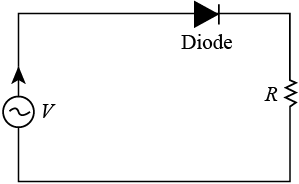
\includegraphics[scale=0.6]{media/Rectifier Circuit.png}
    \caption{A simple half-wave rectifier circuit.\protect\footnotemark}
\end{figure}
\footnotetext{Source: \url{https://homework.study.com/explanation/what-is-a-rectifier-circuit.html}}

Consider the case of a sinusoidal alternating current. If the first half cycle acts in the forward-biased direction of the diode, current flows round the circuit, creating a potential difference across $R$ which will have almost the same value as the input potential difference $V$. During the second half cycle, the diode is reverse-biased, hence little or no current flows in the circuit and the potential difference across $R$ is zero. The current is unidirectional and so the potential difference across $R$ is direct, for although it fluctuates, it never changes direction.

\begin{figure}[H]
    \centering
    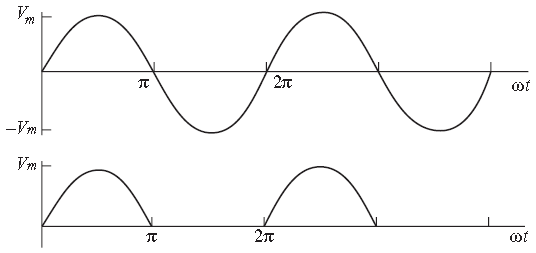
\includegraphics[scale=0.5]{media/Half-Wave Rectifier - Graph.png}
    \caption{The graphs of the input potential difference $V$ and the potential difference across $R$ over time.\protect\footnotemark}
\end{figure}
\footnotetext{Source: \url{https://www.researchgate.net/publication/344782988_Electronic_trainer_for_educational_purposes}}